% Chapter 1

\chapter{Introduction} % Main chapter title

\label{Chapter1} % For referencing the chapter elsewhere, use \ref{Chapter1}

%----------------------------------------------------------------------------------------

% Define some commands to keep the formatting separated from the content
\newcommand{\keyword}[1]{\textbf{#1}}
\newcommand{\tabhead}[1]{\textbf{#1}}
\newcommand{\code}[1]{\texttt{#1}}
\newcommand{\file}[1]{\texttt{\bfseries#1}}
\newcommand{\option}[1]{\texttt{\itshape#1}}

%------------------------------------------------------------------
%------------------------------------------------------------------

\section{Background}

Computer Vision (CV) has jumped by leaps and bounds in the last five years as machine learning, notably deep convolutional neural networks, have become a driving force for pushing the bounds on tasks such as classification, segmentation, and object detection. Industry has jumped on the deep learning wave and today you can purchase products which use facial recognition for security, ride in vehicles that operate autonomously in complex safety critical environments, or get a cancer diagnosis more accurate then seasoned doctors from a machine \cite{Cancer}.

In parallel to advances in computer vision micro-UAVs, colloquially referred to as drones, have found there way out of research labs and into the hands of consumers and professions a like. As demand for drones has built we have seen a steady increase in capabilities with regards to stability, vehicle configuration, flight duration, payload options and autonomy.

One area that is consistently under served by emerging technologies are ecology and conservation. Both areas have ample need for these technologies which can enable scientists access to the information needed to gain new insights into complex environments that are seeing rapid change due to climate change and habitat loss. In this research we show a pipeline see ~\ref{fig:Pipeline} for collecting very high resolution aerial imagery from UAVs, pre-processing the imagery into an orthomosaic using commercial GIS software, and finally using deep convolution neural networks to accurately identify individual species of trees in rain forest canopies. We show that this fine grained classification is only possible with superior than satellite resolution and it has the ability to generalize to new sites with different lighting conditions and resolutions. This study directly enabled ecologists to pull useful insights from our study area.

\begin{figure}[ht]
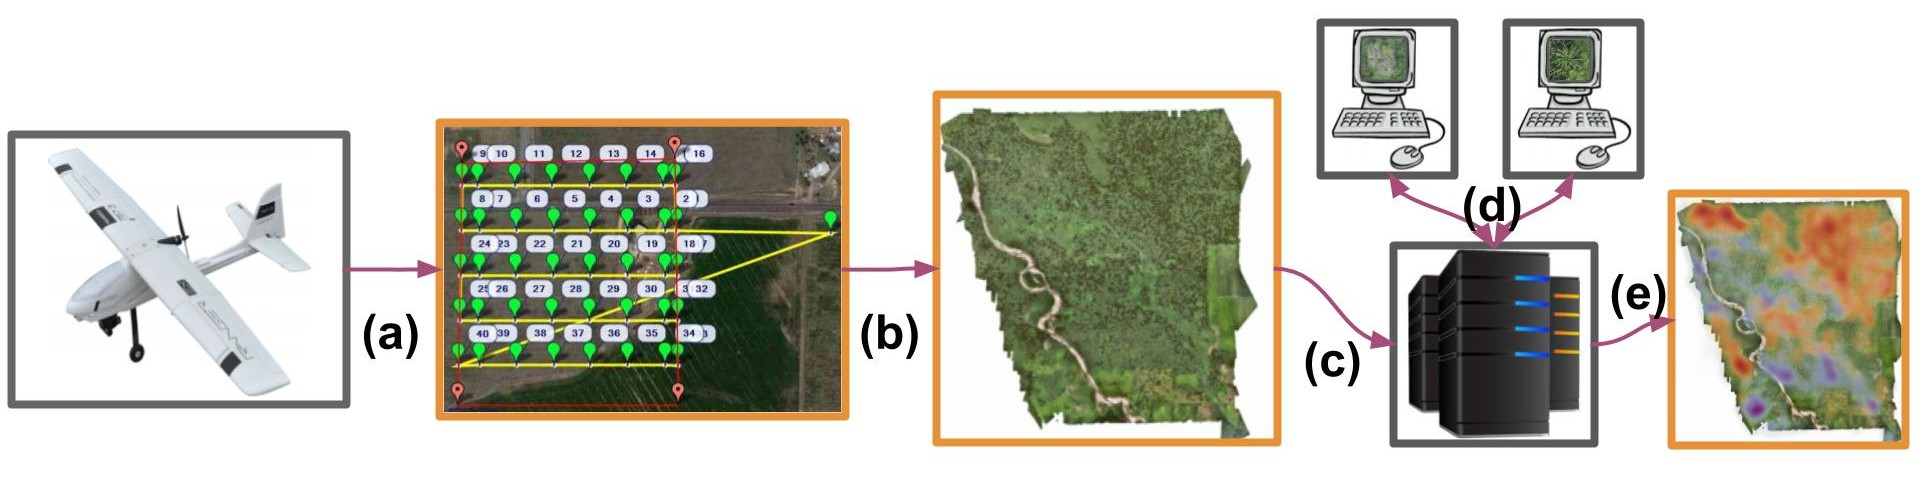
\includegraphics[width=1.0\textwidth]{Figures/Pipeline.jpg}
\caption{\textbf{Data Processing Pipeline.} a) UAV flies a lawn mower flight pattern taking pictures at regular intervals. b) The raw images with GPS and orientation information are stitched together to create an orthomosaic of the canopy; covering about 8.73km2 of data at the BFREE site. c) Orthomosaic is split into smaller images and stored on a server for labeling. d) Web based tool distributes a small subset of the images to volunteers who label them to provide “ground truth”. e) CNN uses the ground truth data train a classifier to detect ecological features (e.g., a specific type of tree). This classifier is used to process the remaining data and automatically characterize the images and orthophoto.}
\label{fig:Pipeline}
\end{figure}

%------------------------------------------------------------------
%------------------------------------------------------------------

\section{What is Deep Learning?}

Deep Learning is an aspect of machine learning that is currently very popular for a variety of tasks, such as natural language processing, computer vision, and even control. Traditionally for each of these disciplines researchers would posit a model that tried to capture the underlying truth of how the world works. For natural language processing this might be how consonants and vowels are related to each other; how different parts of a sentence are connected and influence the overall semantic meaning. For computer vision it might be how edges, contours or colors make up an object such as a dog or cat. For the most part these largely hand designed models fail to capture the entire underlying model which might be highly nonlinear in nature.

This is where neural networks step in as universal function approximaters. Neural networks are formed by an input layer, hidden layer(s), and an output layer. Each node is like a neuron and is connected to other nodes much like the synapses of biological systems. The systems are trained by providing training examples and comparing the output with the desired output and then performing back-propagation to push the parameters of the network towards a better solution. The upshot of these networks are that they are model free reducing the burden on the engineer or scientist to create one by hand. The downside is that they often require massive amounts of data before they perform well, can be computationally expensive, and are largely black boxes that are difficult to inspect. For computer vision the most popular deep learning algorithm has been convolutional neural networks (CNN) which we will utilize as powerful tool for automating perception tasks in ecology and conservation.

\subsection{Brief background to CNNs}

Using computer algorithms to detect and classify objects in digital images is an intrinsically hard problem that has eluded computer vision experts best attempts to model for years. Retaining the 2D structure of an object in an image and discerning how semantic parts of it relate to each other in any given orientation or position is no small feat.

A big step forward came in 2012 when Alex Krizhevsky proposed a learning algorithm that is loosely inspired by how the human visual cortex system works \cite{AlexNet}. It uses many stacked layers of 2D convolutional filters along with nonlinear activation layers to form a neural network capable of learning complex hierarchical representations of objects. While the idea itself wasn't novel idea (neural networks have been around for decades) his use of the massively parallel computation available in graphic processing units (GPUs), deeply stacked layers, and massive amounts of training data allowed him to score $10.8\%$ better than the nearest computation; a huge break through in accuracy. Krizhevsky’s neural network called “AlexNet” is largely considered a silver bullet that helped computer vision researchers overcome a barrier in classification accuracy that they had been running up against for years and leading to a overall boom in deep learning research.

CNNs are a very active area of research and at this point AlexNet is considered outdated. Today Residual network (ResNet) \cite{ResNet} and Densely Connected Convolutional Networks (DenseNet) \cite{DenseNet} are the top performing networks that form the backbone for other problems like object detection, segmentation, and pose regression.

\subsection{Object Detection}

A subset of Deep Learning networks for computer vision are called object detectors. These networks deal with not only classifying an image, but first localizing an individual object in an image frame before assigning it a classification as well as a confidence. Many open source variants of object detectors exist with various strengths and weakness. We considered two algorithms for object detection and recognition: Faster-RCNN and YOLOv2. Faster-RCNN \cite{FASTER-RCNN} uses two networks where the first network proposes a “region” while the second network classifies that region.  YOLOv2 \cite{YOLOv2} uses a single unified network that simultaneously predicts location and class. They both use open source GPU frameworks Caffe and Darknet respectively.  While the two networks are comparable in accuracy on standard datasets, we found that YOLOv2 had the advantage when working with high resolution imagery as it can accept arbitrarily large input images. This is unlike many neural networks where the input size is fixed and makes detection of small objects in high resolution imagery harder due downsampling an image before passing it through the network.

%------------------------------------------------------------------
%------------------------------------------------------------------

\section{Why Ecology and Conservation?}

Macro understanding of ecosystems are usually done by making assumptions based on \textit{macro} features instead of fine grained details. For example forests are usually classified into broads types: coniferous, evergreen, tropical, or mediterranean instead of the individual species that make up the forest. Population counts of arctic fur seals are done with boots on the ground. Coral reef classification is done exhaustively by hand on only small sections at a time. The more fine grain the examination the more labor intensive the process which leads to a loss in temporal coherence as such tasks are only performed rarely and at much greater cost. Ideally researchers would be able to obtain fine-grain temporally coherent analysis of ecosystems without having to invest large amounts of time and money. This is where computer vision can jump in.

\subsection{What does Computer Vision offer Ecologists?}

A few tasks that researchers need to perform such as counting populations of individuals species, marking geographical distribution of individuals, or even identification of individuals in a population are quite easy for humans but traditionally very difficult to automate with machines. The promise and hype around much of the capabilities surrounding deep learning is underlied by the idea that given enough training data we can teach machines to operate at and even above human level abilities for certain tasks. Applying these emerging technologies can allow researchers to automate many processes that can be too labor intensive to do manually.

This technology has already begun to seep into conservation projects. For example Right Whale classification and individual IDing was presented in Kaggle competition by NOAA \cite{DeepSense}. In a similar sense the authors of \cite{Gorilla} used an object detector with facial recognition to find and ID gorillas in the wild. The authors in \cite{GoogleTrees} leveraged Google Street View and Google Earth satellite imagery to classify trees, geo-locate them, and estimate trunk thickness. Researchers from both engineering and ecology are just beginning to jointly explore computer vision tools for these types of challenging tasks.

%------------------------------------------------------------------
%------------------------------------------------------------------

\section{Why UAVs?}

Taking to the sky has always been a force multiplier for mankind and few things have put flight into peoples hands as cheaply as micro unmanned aerial vehicles which we will interchangeable call UAVs, MAVs, or drones. In the consumer world UAVs are more commonly referred to as drones and come in a price range from sub fifty dollar toys designed to be flown inside by children to multi-thousand dollar aircraft for taking action videos. They have been successfully commercialized and used by government organizations to: survey land, create 3D reconstructions of building, monitor agricultural crops, perform remote inspection on wind turbines, assistant in search and rescue, and even provide broadband coverage during natural disasters to name a few.

\subsection{Types of UAVs}

The two most common platforms are multi-rotor copters and fixed wing planes.

Multi-rotor copters usually consist of three to eight propellers, commonly four (quadcopters), with battery, electronics and payload centered on the vehicle. They range in size from as small as ten centimeters to several meters for the largest platforms. Their popularity comes from their ability to move in six degrees of freedom and their ease of flying; making it an ideal platform for inspection and shooting video. They aren't very aerodynamically efficient and usually have flight durations ranging from 10-45 minutes depending on configuration and payload. They are often very weight constrained limiting the types and sizes of payloads they are capable of carrying.

Fixed wing planes are essentially miniaturized versions of manned planes we are accustomed to seeing in our skies. Just like traditional aircraft they come in a large variety of shapes and sizes that have different advantages in flight duration, agility, payload capacity, etc... They vary from hand launched, to shot runway takeoffs, to being catapulted by pneumatic machines. The advantage to fixed wing aircraft are that they are much more efficient than multi-rotor copters with increased payload capacity, longer flight durations, and faster speeds.

For conservation in ecology both vehicle types have important use cases. For our research focusing on wide-scale classification of rain forest canopies a fixed wing aircraft was a natural choice for its long range capabilities.

\subsection{Autopilots}

At the heart of most MAVs are highly sophisticated autopilot systems that use inertial measurement units, GPS, and embedded processors capable of handling low level control/stabilization as well as high level decision making. Prior to a decade ago autopilots with these capabilities were extremely expensive and not commercially available. As cheap micro electronic measurement sensors (MEMS) and faster embedded processors made their way onto the market they began to find their way into autopilots. This is at the heart of the explosion of UAVs on the market. Today they are many autopilots with many available as open source, open hardware projects which are ideal for research applications.

Autopilots usually operate in two different modes: fully autonomous and fly-by-wire. In fly-by-wire mode the autopilot sits between the human and the aircraft to stabilize the vehicle and make the end task for the human much easier. All multi-rotor vehicles operate in this manner. In fully autonomous mode the vehicle has a high level mission plan from the user which commonly consists of a set of waypoints and actions to perform at those waypoints. In this research we make heavy use of this waypoint following to automate the flight paths and image capture in order to achieve a certain amount of overlap per image.

\subsection{What do UAVs offer Conservationists?}
